\subsection{NFV Architecture}

The goal of NFV  is to be able to run network services traditionally hosted in specialized hardware in virtualized resources like virtual machines and containers. This gives the necessary flexibility for realizing use-cases discussed above.  The following figure shows the reference architecture of a typical NFV deployment. The essential framework is outlined by etsi at \cite{etsi02}.

\begin{figure}[h!]
	\centering
	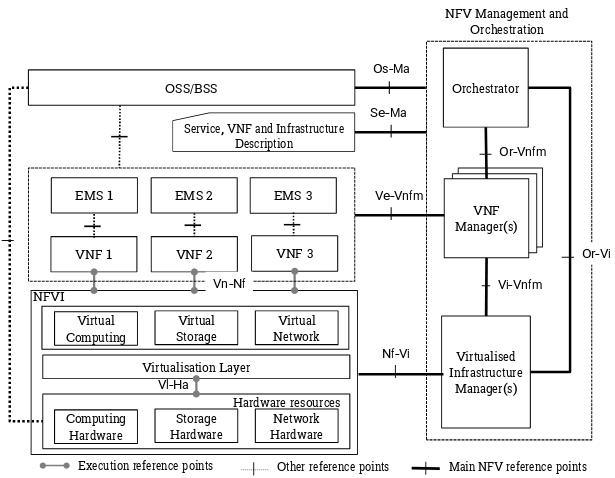
\includegraphics[width=0.9\textwidth]{nfv_ref_architecture}
	\label{fig:figure5}
    \caption{ETSI NFV Reference Architecture \cite{etsi02}}
\end{figure}

The NFV Architecture Framework in~\ref{fig:figure5} is a reference for designing an NFV solution and proposes the following components:

\begin{enumerate}
    \item \textit{Virtual Network Function}
        The functionality that traditionally runs on dedicated hardware and is intended to be virtualized. The functions could be the basic Enterprise functions like Firewall, DNS etc or specialized telecommunication functions like packet processing, mobility management etc,. The VNF can run on a single entity like a virtual machine or a container or on a cluster of virtual machines or containers. The functions that use containers as compute resources are sometimes referred to as Containerized Network Functions (CNF). 
    \item \textit{Element Management}
        The Element Management unit can be used to manage single of multipl VNF units for combined functionality. 
    \item \textit{NFV Infrastructure}
        NFVI refers to the virtualization infrastructure resources providing the compute, network and storage requirements of the VNFs. The infrastructure could comprise of Virtual Machines or Containers, Block and Object Storage units, Network artifacts and the hardware resources that hosts these resources.   
    \item \textit{Virtualized Infrastructure Manager}
        The VIM provides the management functions for the virtualized infrastructure. The functions include inventory management, resource allocation, monitoring, capacity planning, fault management, resource optimization and policy management.
    \item \textit{NFV Orchestrator}
        The Orchestrator is responsible for translating the requirements of a VNF into corresponding resources on the Virtualized Infrastructure. A standard format of description can be used for describing the requirements that can be answered by different VIM solutions.
    \item \textit{VNF Manager}
        The VNF Manager manages the lifecycle of the VNF including instantiation, update, query, scaling, termination and service availability
    \item \textit{Service, VNF and Infrastructure Description}
        This describes a model to describe the entities in the NFV architecture including the Service, VNF and the Infrastructure. The model should be standard and universal so that the same description can be used to abstractly realize multiple types of infrastructure solutions. 
    \item \textit{Operations and Business Support Systems - OSS/BSS}
        The Orchestration and Management blocks of the NFV reference architecture are expected to expose standard APIs for applications. The set of applications that monitor and collect various measurement data from the NFV system can also provide for operational and business functions like service provisioning, billing, auditing etc,. that are essential functions for an operator in order to monetize the solution offered through NFV.
\end{enumerate}
